{\bf Problem format was changed from original. Problem now have 15 seconds timelimit instead of unlimited interaction with environment and grader instead of library. }

В игру <<черный ящик>> играют с помощью квадратного черного ящика, который располагается на плоском столе. На каждой из сторон ящика есть $n$ отверстий (всего $4\cdot n$ отверстий, причём $1 \le n \le 30$), в которые можно вбрасывать шар. Вброшенный шар через некоторое время вылетит наружу через одно из $4\cdot n$ отверстий, возможно, через то же отверстие, в которое он был вброшен.

Содержимое черного ящика можно рассматривать в виде сетки размером $n \times n$. Отверстия в сторонах ящика -- это начала и концы строк и столбцов сетки. Каждая клетка сетки либо пустая, либо занята отражателем. Отражатель -- это устройство, которое изменяет направление движения шара на $90$ градусов. Рассмотрим пример ящика размером $5 \times 5$.

\begin{center}
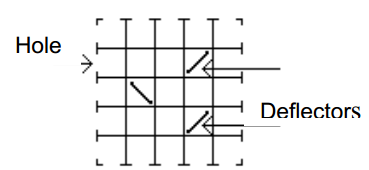
\includegraphics[bb=0 0 275 120]{blackbox1.png}
\end{center}

Вброшенный шар движется по прямой, пока не попадает в отражатель или не вылетит наружу. Когда шар попадает в отражатель, шар меняет направление своего движения, а отражатель меняет свое положение (под словом <<меняет>> подразумевается поворот на $90$ градусов). На примере показаны действия отражателя.

\begin{center}
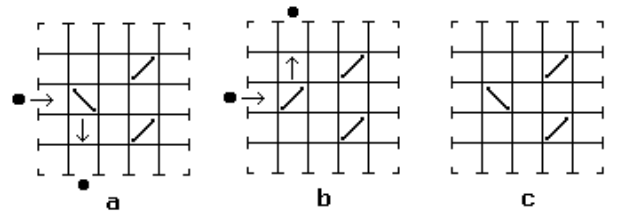
\includegraphics[bb=0 0 600 150]{blackbox2.png}
\end{center}

\begin{enumerate}
\item Первый шар вброшен через отверстие. Он попал в отражатель и изменил направление движения.
\item После попадания первого шара отражатель изменил свое положение. Новый шар вбросили в то же отверстие, он попал в тот же отражатель, и отразился в направлении, противоположном направлению первого шара после отражения.
\item Отражатель изменил свое положение. После каждого попадания положение отражателя изменяется.
\end{enumerate}

Когда шар попадает в отражатель, раздается звуковой сигнал. Количество отражений шара можно узнать, посчитав количество сигналов. Можно доказать, что шар всегда вылетает из ящика. У ящика есть одна кнопка, которая приводит его в исходное положение, и другая кнопка, которая меняет положение всех отражателей на противоположное.

Вам будет предоставлен доступ к черному ящику через грейдер. Вы должны определить внутренности коробки как можно лучше.